\documentclass[convert]{standalone}


\usepackage{tikz}
\usepackage{ifthen}

\tikzstyle{dots}=[%
	every node/.style={
		circle, inner sep = 0, fill=black, minimum size = 3pt, anchor=south
	}%
]

\begin{document}
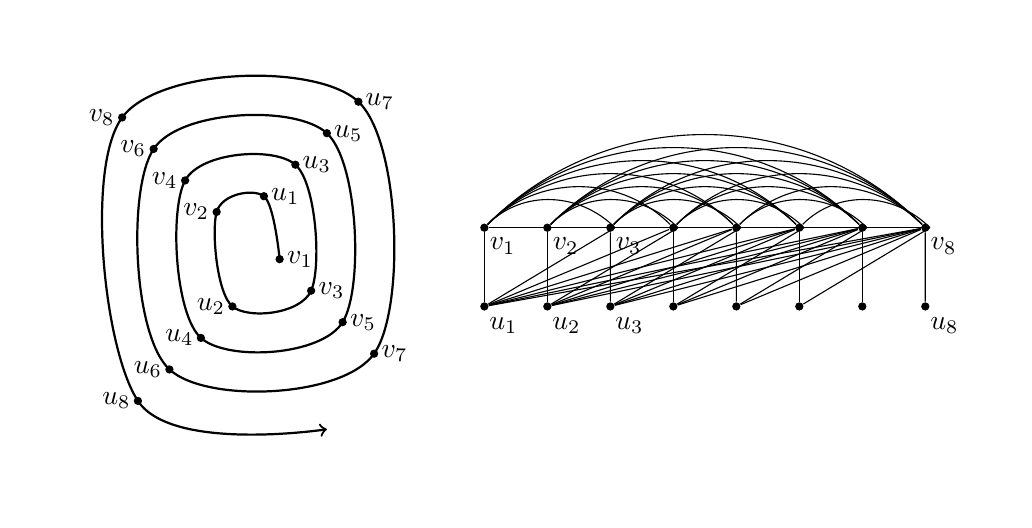
\begin{tikzpicture}[scale=0.2, dots]
	\draw[fill=white, draw=none] (-14,-17) rectangle ++(62,30);

	\node[label={right:{$u_1$}}] (u1) at (1,2)  {};
	\node[label={right:{$u_3$}}] (u3) at (3,4) {};
	\node[label={right:{$u_5$}}] (u5) at (5,6) {};
	\node[label={right:{$u_7$}}] (u7) at (7,8) {};

	\node[label={left:{$u_2$}}] (u2) at (-1,-5) {};
	\node[label={left:{$u_4$}}] (u4) at (-3,-7) {};
	\node[label={left:{$u_6$}}] (u6) at (-5,-9) {};
	\node[label={left:{$u_8$}}] (u8) at (-7,-11) {};
	
	\node[label={right:{$v_1$}}] (v1) at (2,-2) {};
	\node[label={right:{$v_3$}}] (v3) at (4,-4) {};
	\node[label={right:{$v_5$}}] (v5) at (6,-6) {};
	\node[label={right:{$v_7$}}] (v7) at (8,-8) {};
	
	\node[label={left:{$v_2$}}] (v2) at (-2,1) {};
	\node[label={left:{$v_4$}}] (v4) at (-4,3) {};
	\node[label={left:{$v_6$}}] (v6) at (-6,5) {};
	\node[label={left:{$v_8$}}] (v8) at (-8,7) {};

	\draw [thick, black, ->] plot [smooth, tension=0.6] coordinates {
		(v1) (u1)%
		(v2) (u2)%
		(v3) (u3)%
		(v4) (u4)%
		(v5) (u5)%
		(v6) (u6)%
		(v7) (u7)%
		(v8) (u8)%
		(5,-12.5)%
	};

	\begin{scope}[shift = {(11,-5)}]
		\draw[fill=white, draw=none] (1,-4) rectangle (36,9);

		\node[label = {[label distance=2pt] below right:{$v_1$}}] (v1) at ( 4,5) {};
		\node[label = {[label distance=2pt] below right:{$v_2$}}] (v2) at ( 8,5) {};
		\node[label = {[label distance=2pt] below right:{$v_3$}}] (v3) at (12,5) {};
		\node (v4) at (16,5) {};
		\node (v5) at (20,5) {};
		\node (v6) at (24,5) {};
		\node (v7) at (28,5) {};
		\node[label = {[label distance=2pt] below right:{$v_8$}}] (v8) at (32,5) {};

		\node[label = {[label distance=2pt] below right:{$u_1$}}] (u1) at ( 4,0) {};
		\node[label = {[label distance=2pt] below right:{$u_2$}}] (u2) at ( 8,0) {};
		\node[label = {[label distance=2pt] below right:{$u_3$}}] (u3) at (12,0) {};
		\node (u4) at (16,0) {};
		\node (u5) at (20,0) {};
		\node (u6) at (24,0) {};
		\node (u7) at (28,0) {};
		\node[label = {[label distance=2pt] below right:{$u_8$}}] (u8) at (32,0) {};

		\foreach \x in {1,...,6} {
			\draw (u\x) to (v\x);
			\pgfmathsetmacro\ystart{\x+2};
			\foreach \y in {\ystart,...,8} {
				\draw (u\x) to (v\y);
			};
		};
		\draw (u7) to (v7);
		\draw (u8) to (v8);

		\foreach \x in {1,...,6} {
			\pgfmathsetmacro\ypp{\x+1};
			\draw (v\x) to (v\ypp);
			\pgfmathsetmacro\ystart{\ypp+1};
			\foreach \y in {\ystart,...,8} {
				\draw (v\x) to [in=135, out=45] (v\y);
			};
		}
		\draw (v7) to (v8);
	\end{scope}
\end{tikzpicture}
\end{document}








